\documentclass[11pt]{article}
\usepackage{makeidx,graphics}
\usepackage[hidelinks]{hyperref}
\usepackage{amsmath}
\usepackage{latexsym}
\usepackage{amssymb}
\usepackage{array}
\usepackage{amsthm}
\usepackage{graphicx}
\usepackage{epstopdf}
\usepackage{subcaption}
\usepackage{varioref}


\usepackage[margin=1in]{geometry}

\theoremstyle{plain} 
\newtheorem{Thm}{Theorem}[section]
\newtheorem{Cor}[Thm]{Corollary}
\newtheorem{Lem}[Thm]{Lemma}
\newtheorem{Prop}[Thm]{Proposition}
\newtheorem*{Thm*}{Theorem}

\theoremstyle{definition}
\newtheorem{Def}[Thm]{Definition}
\newtheorem{Rem}[Thm]{Remark}
\newtheorem{Exa}[Thm]{Example}
\newtheorem{xca}{ }[section]
\newtheorem{Prc}{Procedure}[section]
\newtheorem*{Def*}{Definition}
\newtheoremstyle{Nmthm}% name
  {3pt}           % Space above, empty = `usual value'
  {3pt}           % Space below
  {\itshape}      % Body font
  {}              % Indent amount (empty = no indent, \parindent = para indent)
  {\bfseries}     % Thm head font
  {.}             % Punctuation after thm head
  {.5em}          % Space after thm head: " " = normal interword space;
                  % \newline = linebreak
  {\thmnote{#3}}  % Thm head spec

\theoremstyle{Nmthm}
\newtheorem*{Nmthm}{} % all text will be supplied in the note



\begin{document}

% double spacing
\setlength{\baselineskip}{22pt}

% title page
\title{Neural Networks}
\author{Catalina Vajiac\\
Advisor: Chris Wedrychowicz}

\date{\today}
\maketitle

\newpage
\tableofcontents

\pagenumbering{arabic}

% chapters
\newpage
\section{Introduction}

The goal of image classification is to determine the main contents of an image,
commonly referred to as the image's \textit{class}. This is a more complex
problem than one may think when first studying it due to the variation in
images. While there are many algorithms that attempt to classify images, neural
networks are known to be most successful in doing so.

There are many different cases in which one can have an unideal image,
including viewpoint variation, scale variation, deformation, occlusion,
illumination conditions, and intra-class variation. These will be described in
detail later on in this paper, but they all describe ways in which images of
the same class can vary. For this reason, a complex algorithm is required to
classify images.

Neural networks classify images using a data-driven approach by processing many
examples from different classes of images. They have neurons, or units, that
learn the features of a dataset. Those units then propagate information to
other units. This process allows the algorithm to learn from observational
data.

Neural networks have two phases; training and inference. In the training phase,
they learn from a large dataset, and in inference, they apply that knowledge to
new testing data that hasn't been seen before. There's a rich mathematical
theory involved in designing a neural network, which will be described in
detail in Chapter \ref{ch:gradient_descent}.

Despite advances in hardware that have made it feasable to use neural networks,
they are still extremely computationally expensive to train, sometimes taking
weeks or months to do so. Current research is being conducted in order to find
ways to speed up neural networks by innovative technical companies, such as
Google, Facebook, and AMD. While it is not the focus of this paper to discuss
this topic, it's important to realize that new techniques are still being
developed as this is a growing field.

In Sections \ref{ch:image_classification} and \ref{ch:neural_networks}, we will
discuss background for image classification and neural networks. In Section
\ref{ch:gradient_descent}, gradient descent, the iterative algorithm that
trains a neural network will be discussed. In Section \ref{ch:python}, we will
discuss the implementation of a fully-connected network in Python.

\newpage
\section{Image Classification}\label{ch:image_classification} Image
classification is a difficult problem to solve because images are usually not
ideal. Common issues with images are described in the
following section.

\subsection{Image Variation} One way that images can differ is by
\textit{viewpoint variation}, or when the same object can be oriented in many
ways with respect to the camera. An example of viewpoint variation is shown in
Figure \ref{fig:viewpoint} below:

\begin{figure}[ht!] \centering
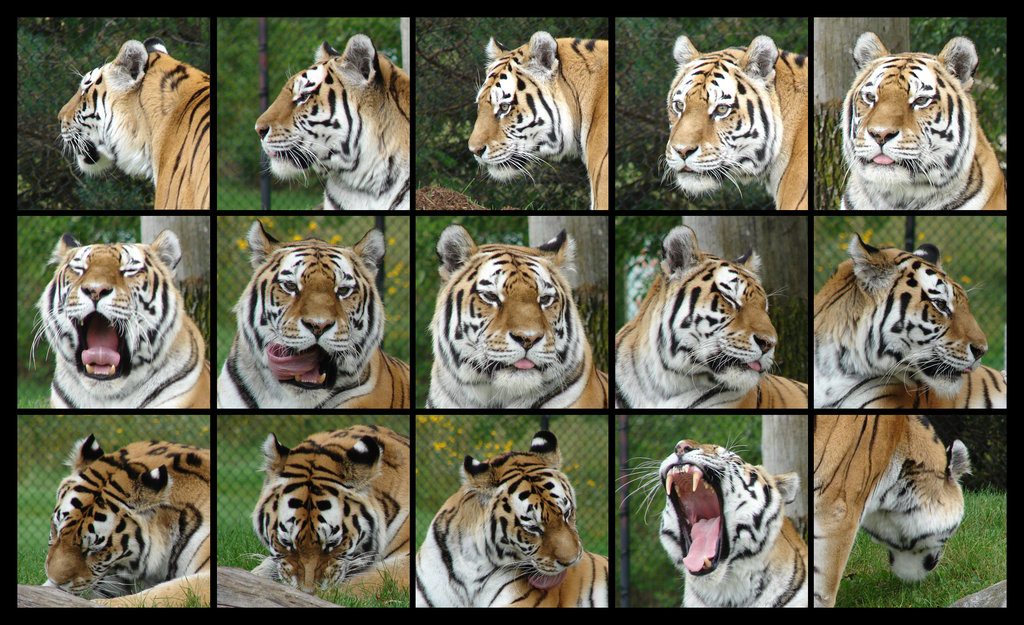
\includegraphics[height=2.5in]{../figures/cat_viewpoint_variation.jpg}
\caption{Tiger's head from many different angles} \label{fig:viewpoint}
\end{figure}

\noindent Above, we see that while each image is very different, our human eye
can detect that we are looking at a tiger. We want an algorithm that can
classify all of these images as a tiger, no matter which direction the image
was taken from.

\noindent Another way in which images can differ is by \textit{scale
variation}, or when there's a difference between sizes of objects within the
same class. Note that this is different than how far away the object is from
the camera when the image is taken; rather, it is more about variation in the
objects themselves.  An example of scale variation is shown in Figure
\ref{fig:scale_variation} below.

% FORMATTING
\newpage

\begin{figure}[ht!] \centering

\includegraphics[height=2.5in]{../figures/kitty_scale_variation.jpg}
\caption{Scale variation with cats.} \label{fig:scale_variation} \end{figure}

\noindent We note that, while all of these animals can be classified as cats,
they look quite different. Two of the cats are very small and one of the cats
is significantly larger. This kind of variation occurs regularly within
classes, and it implies that we cannot use the size of an object or its size
relative to other objects as a way to determine its class.

\noindent Objects in an image can also be \textit{deformed}. Since objects of interest
are often not rigid, their shape can vary in many ways. An example of
deformation is shown in Figure \ref{fig:deformation} below.

\begin{figure}[ht!] \centering
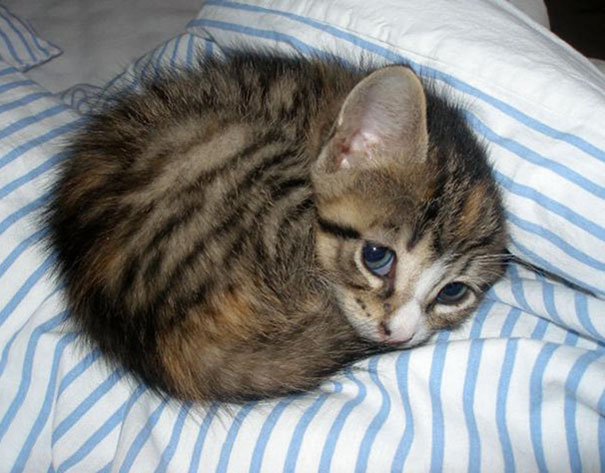
\includegraphics[height=2.5in]{../figures/kitty_deformed.jpg}
\caption{Deformation with cats.} \label{fig:deformation} \end{figure}

\noindent Above, we see that while cats usually have a very specific shape with
protruding legs and tail, this cat is curled up and does not clearly show those
features.

\noindent Sometimes objects in an image can be \textit{occluded}, so only part
of the object is visible. An example of oclusion is shown in Figure
\ref{fig:occlusion} below.

\begin{figure}[ht!] \centering

\includegraphics[height=2.5in]{../figures/kitty_occlusion.jpg}
\caption{Occlusion with cats.} \label{fig:occlusion} \end{figure}

\noindent In this image, only the head and two paws of the kitten is visible.
The back two paws, the tail, and most of the kitten's body is hidden, which
makes it harder to classify.

\noindent This image also has another issue known as \textit{background
clutter}. Not only is the cat occluded, but it's surrounded by objects of a
similar color.  From the algorithm's perspective, it can be it difficult to
separate an image's subject from its background.

\noindent Illumination conditions greatly change the pixel values of an image
and sometimes make it difficult to see the object to be classified. An example
of this is shown in Figure \ref{fig:illumination} below.

\begin{figure}[ht!] \centering

\includegraphics[height=2.5in]{../figures/kitty_illumination.jpg}
\caption{Illumination conditions with cats.} \label{fig:illumination}
\end{figure}

\noindent In this iamge, there's a very stark contrast between the cat and its
background.  Different lighting conditions can also make an object appear more
yellow, more blue, or very dark, which can make it harder to classify.

\noindent Classes of interest can be relatively broad, meaning there's not one
specific way that an object of that class should look like.  This issue is
referred to as intra-class variation. An example of this is shown in Figure
\ref{fig:intra_class_variation} below.

\begin{figure}[ht!] \centering
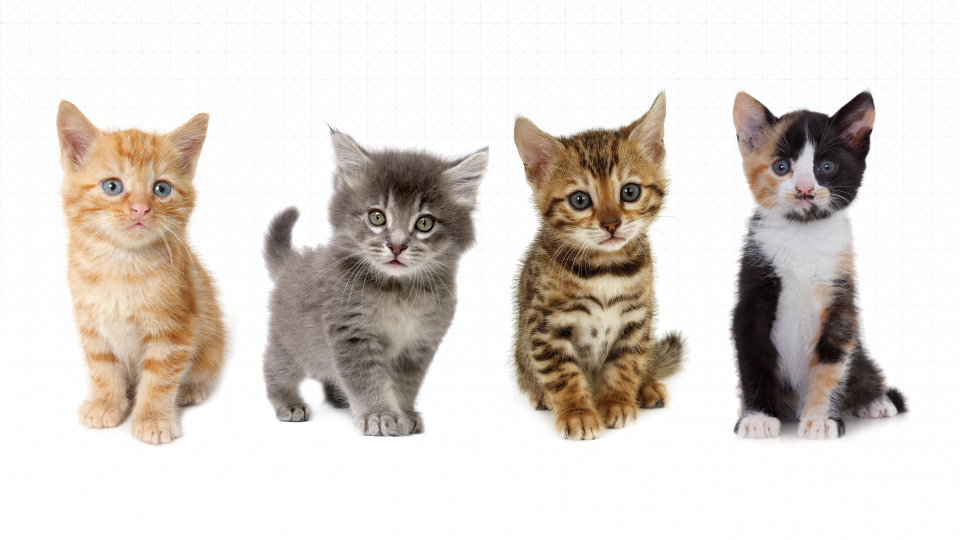
\includegraphics[height=2.5in]{../figures/kitty_intra_class_variation.jpg}
\caption{Intra-class variation with cats.} \label{fig:intra_class_variation}
\end{figure}

\noindent Because there is a generally a large amount of variation between
images of the same class as described above, it is not obvious as to how one
would write an algorithm for identifying a specific class within an image.
Instead of specifying what the features for every class might be, we will
instead take a data-driven approach, where we give an algorithm many examples
of each class and allow it to look at those examples and learn what objects of
each class look like, just like a child would do when seeing new objects for
the frist time. This is exactly what neural networks accomplish.

\subsection{Common Datasets for Neural Networks}
To test my implemented network, I looked at two different image classification
datasets; MNIST and CIFAR10. MNIST is a database of images of handwritten
digits 0-9, with the goal being to classify which digit the image represents.
All images in MNIST are $28\times28$ pixels and greyscale.

CIFAR-10 is an object classificaiton dataset. All images in CIFAR-10 are 32x32
pixel images with three color channels: red, green, and blue. This dataset is
generally a more difficult problem to solve than MNIST since the images are
fully colored, meaning there is more data to process, and there's also more
variation between the images in the dataset.

\newpage
\section{Neural Network Architectures}\label{ch:neural_networks}
There are a many different types of neural network architectures. We will talk
about fully-connected, deep, and convolutional neural networks. Some of these
architectures are simpler to implement in practice than others and lend
themselves better to certain types of problems. Remember that image
classification is not the only problem that neural networks are able to solve.

\subsection{Fully-Connected Neural Network} A fully-connected neural network is
a network where all units in one layer are connected to all units in the
following layer. A nonlinear neural network has at least three layers: an input
layer, a hidden layer, and an output layer. Units in the input layer correspond
to the inputs fed into the network. In the case of image classification, this
corresponds to the pixels within each training example.  The output layer's
units correspond to the number of classes an image could fall under. In the
case of both MNIST and CIFAR-10, this number is 10.  A visualization of the
structure of a neural network is shown in Figure \ref{fig:nn} below.

\begin{figure}[ht!]
\centering
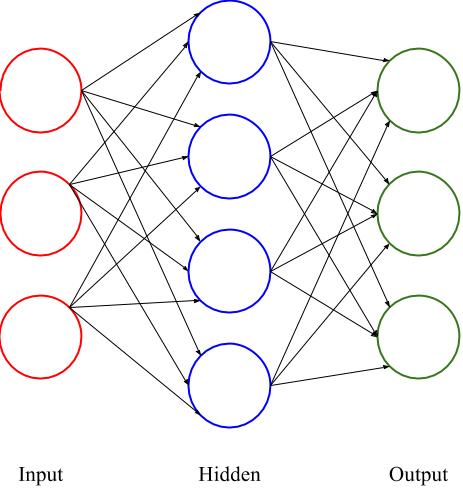
\includegraphics[height=3in]{../figures/neural_network.png}
\caption{Visualization of a fully-connected network.}
\label{fig:nn}
\end{figure}

\subsection{Deep Neural Network}
A neural network can have multiple hidden layers. If it does, it is then
referred to as a deep neural network (DNN). An visualization of a DNN is shown
below.

\begin{figure}[ht!]
\centering
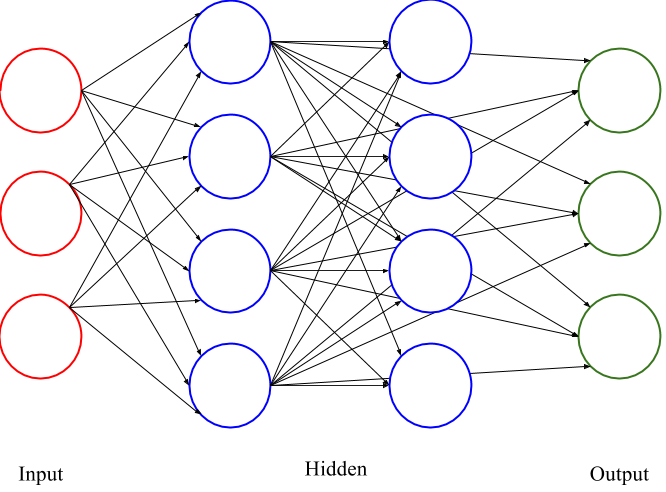
\includegraphics[height=3in]{../figures/deep_nn.png}
\caption{Visualization of a DNN}
\label{fig:dnn}
\end{figure}

We will go into the theory explaining what information each layer of the
network is propogating and explain why multiple layers can achieve better
performance in Chapter \ref{ch:gradient_descent}, but for now, we note that
with multiple hidden layers, information about the images will be learned more
accurately for each iteration of the Gradient Descent algorithm, which is the
algorithm on which a neural network trains. We will discuss this algorithm in
detail later.

\subsection{Convolutional Neural Network}
A convolutional neural network (CNN) is a network where not all units in one
layer are connected to all units in the next. Not all pixels in an image give
useful information about every part of the object they are trying to classify,
so CNNs are commonly used for image classification. They try to avoid
unnecessary computation by removing interactions between units that aren't
providing useful information to each other. A visualization of the structure
of a convolutional neural network is shown in Figure \ref{fig:cnn} below.
\newpage
\begin{figure}[ht!]
\centering
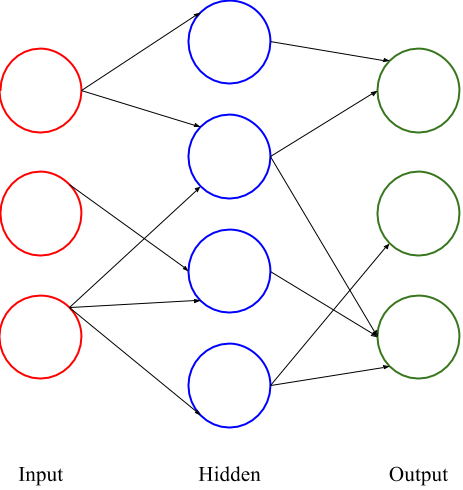
\includegraphics[height=3in]{../figures/convolutional_nn.png}
\caption{Visualization of a CNN}
\label{fig:cnn}
\end{figure}

Note that a CNN can also be a DNN if there are multiple hidden layers. For
image classification, convolutional neural networks tend to perform the best.

\noindent Due to time constraints, this paper will focus exclusively on fully connected
neural networks.

\newpage
\section{Gradient Descent}\label{ch:gradient_descent}

%explain batches

%explain weights, that weights change after a batch props, not whole network

\subsection{Linear Classification}

Suppose our training data is represented by a matrix $X$ which has dimensions
$m \times n$, meaning there are $m$ examples, each with $n$ features. Let us
suppose that each piece of data in $X$ belongs to one of $k$ classes, and the
labels corresponding to each example are stored in a matrix $y$ which has
dimension $m \times k$, where each row of $y$ contains a one in the column
corresponding to the class which that example corresponds to, and zeros
everywhere else.

Suppose that we have a matrix $W$ with dimension $n \times k$ and a vector $b$
of dimension $k \times 1$. We can build a prediction matrix $P$ where

\[
P = XW + b.
\]

Note that we must broadcast $b$ to an $m \times k$ matrix to compute this sum.
Each row of $P$ contains $k$ scores, which each represent how closely that
training example matches each class. A prediction can be made by predicting the
class which corresponds to the entry of the highest score. The accuracy of
these predictions can be evaluated with respect to the class labels found in
$y$.

We will now discuss how to determine $W$ and $b$ given our training data $X$
and its labels $y$. The goal of training a softmax classifier is to determine
the optimal values for these parameters.

\subsection{Loss Functions}

Suppose we have a function $l$ which takes in one training example and its
label data as input and returns some sort of loss for that training example.
The function $L$, defined below, then aggregates the values of $l$ for each
training example. We call this our loss function

\[
L(p, y) = \sum_{i=1}^m l(P_i, y_i),
\]

where $P_i$ denotes the $ith$ row of $P$ and $y_i$ denotes the $ith$ row of
$y$.

We will be looking at the Softmax Loss function, which is defined by

\[
L(P) = -\frac{1}{m} \sum_{i=1}^m \log \frac{\exp{P_{i, y_i}}}
                                           {\sum_{j=1}^k \exp{P_{i, j}}}.
\]

Note that $P$ is dependent on $W$ and $b$, so this can be rewritten as

\[
L(P) = -\frac{1}{m} \sum_{i=1}^m \log
        \frac{\exp{\left(XW\right)_{i, y_i} + b_{y_i}}}
             {\sum_{j=1}^k \exp{\left(XW\right)_{i, j} + b_j}}.
\]

\subsection{Deriving Gradient Update}
We will now work to minimize $L$ by applying gradient descent. The following
will derive the gradient update formula for the Softmax Loss function.

\subsubsection{Deriving $\nabla P$}
We first will determine $\nabla P$ as a step in determining $\nabla W$ and
$\nabla b$. Let us fix a pair of indices $u$, $v$ where $1 \leq u \leq n$ and
$1 \leq v \leq k$. First, we will differentiate with respect to $P_{u, v}$.
Let us fix an $i$ where $1 \leq i \leq m$.  Let $L_i = \frac{\exp{P_{i,
y_i}}}{\sum_{j=1}^k \exp{P_{i, j}}}$.

%Note that \frac{\partial L_u}{\partial P_{u, v} = 0 if $u \neq i$.

Let us also define a matrix $Y$ of size $m \times k$ as $Y_{i, j} = 1(y_i =
j)$. So we have $\frac{\partial L_i}{\partial P_{i,v}} = \sum_{i=1}^m
\frac{\exp{P_{i,v}}}{\sum_{i=1}^k \exp{P_{i,j}}}$.

This makes
\begin{align*}
  \frac{\partial L}{\partial P_{i,v}}
  &= \sum_{i=1}^m \frac{\partial L_i}{\partial P_{i,v}}\\
  &= -\frac{1}{m} Y_{i,v} + \frac{1}{m}
  \frac{\exp{P_{i,v}}}{\sum_{j=1}^k \exp{P_{i,j}}}
\end{align*}
  
since $Y_{i,j}$ only depends on $P_{i,w}$.

Thus $\nabla P_{i,v} = \frac{\partial L}{\partial P_{i,v}} \forall i,v.$

So we have $\partial P_{i,v} = \frac{1}{m} \left[ -Y +
\frac{\exp{P}}{\sum_{i=1}^m \exp{P_i}} \right]$.

\subsubsection{Deriving $\nabla W$}
Now we will derive $\nabla W$ to use in the update step of training. Recall
that $P = XW + b$, meaning $P_{i, j} = \sum_{t=1}^n X_{i, t}W_{t, j} + b_j $.
Also remember that $L_i$ is a function of $P_{u, v}$ only if $u = i$, so it
follows that $\nabla P_{i, j} = \frac{\partial L}{\partial P_{i, j}} =
\frac{\partial L_i}{\partial P_{i, j}}$. The following goes through the
derivation of $\frac{\partial L}{\partial W_{uv}}$.

\begin{align*} 
     \frac{\partial L}{\partial W_{u, v}} = 
     \sum_{i=1}^m \frac{\partial L_i}{\partial W_{u, v}} &= 
     \sum_{i=1}^m \sum_{j=1}^k \frac{\partial L_i}{\partial P_{i, j}}
       \frac{\partial P_{i, j}}{\partial W_{u, v}}\\
     &= \sum_{i=1}^m \sum_{j=1}^k
         \frac{\partial L_i}{\partial P_{i, j}} X_{i, u}\\
     &= \sum_{i=1}^m \frac{\partial L_i}{\partial P_{i, v}} X_{i, u}\\
     &= \sum_{i=1}^m \nabla P_{i, v} X_{i. u}\\
     &= \left( X^T \nabla P \right)_{u, v}.
\end{align*}

Thus, we have
$$ \nabla W = X^T \nabla P. $$

\subsubsection{Deriving $\nabla b$}
We will now derive $\nabla b$ to use in the update step of training. This is
similar to the derivation for $\nabla W$.

We know that $\frac{\partial P_{i,j}}{\partial b_u} = 1(j == u).$
\begin{align*} 
  \frac{\partial L}{\partial b_u} = 
  \sum_{i=1}^m \frac{\partial L_i}{\partial b_u} &= 
  \sum_{i=1}^m \sum_{j=1}^k \frac{\partial L_i}{\partial P_{i, j}}
  \frac{\partial P_{i, j}}{\partial b}\\
  &= \sum_{i=1}^m \sum_{j=1}^k \frac{\partial L_i}{\partial P_{i, j}} 1(j == u)\\
  &= \sum_{i=1}^m \frac{\partial L_i}{\partial P_{i,u}} \\
  &= \sum_{i=1}^m P_{i,u}.
\end{align*}

Thus $\nabla b = \sum_{i=1}^m P_i$.

\subsection{Gradient Descent Update}
Now that we have computer $\nabla W$ and $\nabla b$, we can update $W$
and $b$ by the following:

$$ W = W - \eta \nabla W $$
and
$$ b = b - \eta \nabla b, $$
where $\eta$ is a hyperparameter called the learning rate; it effectively
scales how much parameters will follow the gradient. If $\eta$ is very small,
then the network will take a long time to train, but if $\eta$ is too large,
the network will have trouble finding the optimal $W$ and $b$, which will cause
the training and test accuracies to drop. There are methods for finding optimal
values for $\eta$, but this topic goes beyond the scope of this paper.

At this point, we have enough information to create a Softmax Classifier, which is a
zero-layer neural net. (Note: recall that when we refer to the number of layers
a neural net has, we refer to the number of hidden layers)

\subsection{Classifying Non-Linear Data}
The Softmax Classifier is good at classifying linearly separable data. However,
many classification problems involve data that isn't linearly separable. In
order to remedy this, we must add a non-linearity to our neural network
architecture. There are many different ways in which this can be done, but the
current most popular function used to provide non-linearities in neural network
is called the REctified Linear Unit (RELU) function, and is defined as follows:

\[ relu(x) = \begin{cases} 
      0 & x\leq 0 \\
      x & x > 0 
   \end{cases}
\]

\subsubsection{Deriving $\nabla X$}

\subsection{One Layer Neural Net}

\newpage
\section{Implementation in Python}\label{ch:python}

\newpage
\section{Other Network Features}\label{ch:other_features}
% dropout, batch normalization, etc


% bibliography
\bibliographystyle{siam}
\nocite{*}
\newpage
\bibliography{chapters/bibliography}

%\appendix
%\section{Definitions}
\end{document}
